\documentclass{standalone}
\usepackage{tikz}
\usepackage{ctex,siunitx}
\setCJKmainfont{Noto Serif CJK SC}
\usepackage{tkz-euclide}
\usepackage{amsmath}
\usetikzlibrary{patterns, calc}
\usetikzlibrary {decorations.pathmorphing, decorations.pathreplacing, decorations.shapes,}

\begin{document}
\small
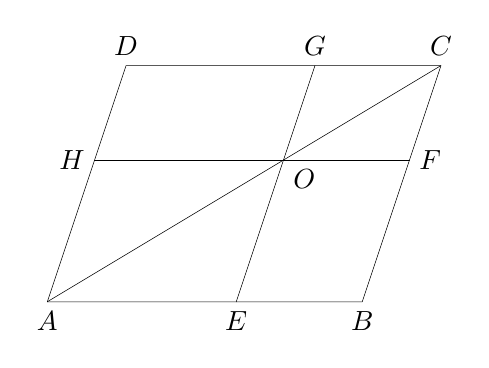
\begin{tikzpicture}[>=stealth,scale=1.0]
  \tkzSetUpPoint[fill=black]
  % \useasboundingbox(-1,-0.75)rectangle(3.7,1.4);
  \tkzDefPoints{0/0/A, 4/0/B, 5/3/C}
  \tkzDefPointsBy[translation = from B to C](A){D}
  \tkzDefPointWith[linear, K=.6](A,C) \tkzGetPoint{O}
  \tkzDefPointWith[linear, K=.6](A,D) \tkzGetPoint{H}
  \tkzDefPointWith[linear, K=.6](B,C) \tkzGetPoint{F}
  \tkzDefPointWith[linear, K=.6](D,C) \tkzGetPoint{G}
  \tkzDefPointWith[linear, K=.6](A,B) \tkzGetPoint{E}
  \tkzDrawPolygon(A,B,C,D)
  \tkzDrawSegments(A,C H,F G,E)
  \tkzLabelPoints[below](A,E,B)
  \tkzLabelPoints[above](D,G,C)
  \tkzLabelPoints[left](H)
  \tkzLabelPoints[right](F)
  \tkzLabelPoints[below right](O)
\end{tikzpicture}
\end{document}